% -*- root: main.tex -*-

\chapter{Loose ends}

---

\todo[inline]{I'd like to spend a couple of days talking about ways the picture in this class can be extended, finally, some actually unanswered questions that naturally arise.  The following two section titles are totally made up and probably won't last.}
\todo[inline]{Also, write a broad-scale introduction to this appendix.}

\section{Orientations by \texorpdfstring{$E_\infty$}{Eoo} maps}



\todo[inline]{What follows is some scaffolding for giving an explicit understanding the $\Spin$ orientation of $KO$ by an $E_\infty$ map, as well as some notes on how the $\String$ orientation of $\tmf$ plays out.  It is not sewn together, or chronologically sound, but I wanted to get the brain-dump down before it's lost.}






A more modern take on the story of the $\sigma$--orientation passes through the algebraic geometry of $E_\infty$--ring spectra, which are the homotopically coherent analogues of commutative ring objects that one finds in the $\infty$--category $\CatOf{Spectra}$.  Essentially all of the ring spectra discussed in this book have incarnations as $E_\infty$--rings:
\begin{theorem}
\citeme{this is a mega-theorem}
The classical $K$--theories $KU$ and $KO$, the Eilenberg--Mac Lane spectra $HR$, the Morava $E$--theories $E_\Gamma$, their fixed point spectra, the Thom spectra arising from the $J$--homomorphism (including $MO$, $MSO$, $M\Spin$, $M\String$, $MU$, $MSU$, and $MU[6, \infty)$), the spectra $\TMF$, $\Tmf$, and $\tmf$ are all $E_\infty$--ring spectra.\footnote{Notably, the Morava $K$--theories are \emph{not} $E_\infty$ rings at finite heights.} \qed
\end{theorem}

A great deal of classical commutative algebra can be lifted into this new setting, including a particular functor \[\gl_1\co E_\infty\CatOf{RingSpectra} \to \CatOf{Spectra}.\]  This functor derives its name from two compatible sources: for one, its underlying infinite loopspace is the construction $GL_1$ described in \Cref{LectureThomSpectra}; and secondly, it participates in an adjunction
\begin{center}
\begin{tikzcd}[column sep=4em]
\CatOf{ConnectiveSpectra} \arrow[shift left=0.3\baselineskip, "\Susp^\infty_+ \Omega^\infty"]{r} & E_\infty\CatOf{RingSpectra} \arrow[shift left=0.3\baselineskip, "\gl_1"]{l}
\end{tikzcd}
\end{center}
analogous to the adjunction between the group of units and the group-ring constructions in classical algebra.  Its relevance to us is its participation in the theory of highly structured Thom spectra.  Let $j\co g \to \gl_1 \S$ be a map of connective spectra, begetting an infinite loopmap $J\co G \to \GL_1 \S$, where we have written $G = \Loops^\infty g$.
\begin{lemma}
\citeme{May? or ABGHR?}
The Thom spectrum of the map $BJ$ is presented by the pushout of $E_\infty$ rings
\begin{center}
\begin{tikzcd}
\Susp^\infty_+ \GL_1 \S \arrow["\Loops^\infty \Susp j"]{r} \arrow{d} & \Susp^\infty_+ \Loops^\infty \gl_1 \S / g \arrow{d} \\
\S \arrow{r} & MG. \qed
\end{tikzcd}
\end{center}
\end{lemma}

\begin{corollary}
\citeme{May, but also ABGHR}
There is a natural equivalence between the space of null-homotopies of the composite \[g \xrightarrow j \gl_1 \S \xrightarrow{\gl_1 \eta_R} \gl_1 R\] and the space of $E_\infty$ ring maps $MG \to R$, where $MG$ is the Thom spectrum of the stable spherical bundle classified by $J$.
\end{corollary}
\begin{proof}
Applying the mapping space functor $E_\infty(-, R)$ to the pushout diagram in the Lemma, we have a pullback diagram of mapping spaces:
\begin{center}
\begin{tikzcd}
E_\infty(\Susp^\infty_+ \GL_1 \S, R) & E_\infty(\Susp^\infty_+ \Loops^\infty \gl_1 \S / g, R) \arrow{l} \\
E_\infty(\S, R) \arrow{u} & E_\infty(MG, R) \arrow{l} \arrow{u}.
\end{tikzcd}
\end{center}
We can reidentify each of the three terms to get
\begin{center}
\begin{tikzcd}
\CatOf{Spectra}(\gl_1 \S, \gl_1 R) & \CatOf{Spectra}(\gl_1 \S / g, \gl_1 R) \arrow{l} \\
\{\gl_1 \eta_R\} \arrow{u} & E_\infty(MG, R) \arrow{l} \arrow{u},
\end{tikzcd}
\end{center}
hence $E_\infty(MG, R)$ appears as the fiber at $\gl_1 \eta_R$ of the restriction map, which coincides with the space of nullhomotopies as claimed.
\end{proof}






\textbf{Question:}  Is it helpful to observe that $\CP^\infty$ rationally \emph{multiplicatively} generates $bSU$, or something like that?





There is the following important logarithm utility calculation:

\begin{theorem}[{\cite[Theorem 4.11]{AHR}}]
Let $R$ be an $E_\infty$ ring spectrum satisfying $R = L_d R$, and set $F$ to be the fiber \[F \to \gl_1 R \to L_n \gl_1 R.\]  Then $\pi_* F$ is torsion and $F$ satisfies the coconnectivity condition $F \simeq F(-\infty, d]$. \qed
\end{theorem}

\noindent from which it follows that $\gl_1 KO_p \to KO_p$ is a $1$--connected map and $\gl_1 \tmf_p \to \tmf_p$ is a $2$--connected map.  So, for the purposes of studying $\String$ orientations, it is safe to follow the logarithm and consider its target as the spectrum under $\gl_1 \S$:













\begin{theorem}[Unpublished work of Hopkins and Lurie]
Let $F_d$ denote the discrepancy spectrum for $E_d$.  There is a natural equivalence of infinite loopspaces $\Loops^\infty F_d \simeq \Susp^d \mathbb I_{\Q/\Z}$. \qed
\end{theorem}

\Cref{OrdinaryHomologyInUpperHalfPlaneEx} is an inspiration for considering $\tmf$ as well.





\subsection{Other things to mention back here}




The $\tmf$ outline is to work by chromatic fracture, comparing $\tmf = L_2 \tmf$ to its $K$--localizations.  There are no maps from $b\String = kO[8, \infty)$ into $L_{K(2)} \tmf$, since $L_{K(2)} kO[8, \infty) = L_{K(2)} kO = 0$.  So, all of the work is in the $K(1)$--local case, either into $L_{K(1)} \tmf$ or $L_{K(1)} L_{K(2)} \tmf$.  One of these is supposed to look like the $p$--adic $K$--theory case (though I'm not sure exactly how) (cf.\ the introduction to the lesser known Ando--Hopkins--Rezk, where they talk about mapping into a $K$--algebra).  The other is supposed to get involved through power operations and the logarithm.  The algebraic picture is supposed to be Katz's monodromy of the $p$--adic moduli of elliptic curves, though it is also not clear to me how.



The ``moments of measures'' picture is pretty nice inside of stable homotopy theory, and it has a nice pedigree (as outlined in the lesser-known AHR).  There they also say that the same picture is crucial in the classical analysis of $p$--adic modular forms, which is worth understanding and describing too.



Haynes's \textit{Universal Bernoulli Numbers} paper is about describing the effect of the $S^1$--transfer in the $MU$--Adams spectral sequence.  The notion is that any convergent spectral sequence can be used to calculate it, and inside of a complex-orientable setting (as for a connected integral complex-orientable spectrum), one can get control over the basics of the Adams spectral sequence by understanding the coaction of $MU_* MU$ on $MU_* \CP{}_{-\infty}^{\infty}$, which is the cofiber of some other (related) transfer.  Unsurprisingly, given all the references, he ends up playing a similar trick to what appears in AHR: he rationalizes $MU$ and studies the difference series $x / \exp_{MU}(x)$ (which specializes in the case of $MU \to KU$ to $x / (1 - e^{-x})$, which is supposed to be where the original Bernoulli numbers appear in the ABS orientation arise).

The Hattori--Stong theorem states that $MU_* \to K_* MU$ has image a direct summand.  Maybe this also deserves mention.  (Baker claims in \textit{Combinatorial and Arithmetic Identities Based on Formal Group Laws} that it has a direct algebraic proof given by Araki in \textit{Typical formal groups in complex cobordism and $K$-theory}.)



\begin{theorem}
The integral $K$--theory cooperations $K_0 K$ are parametrized by rational Laurent polynomials that induce continuous functions $\Z_p^\times \to \Z_p$ for every $p$.
\end{theorem}
\begin{proof}
Consider the $p$--local homotopy pullback square
\begin{center}
\begin{tikzcd}
(K \sm K)_{(p)} \arrow{r} \arrow{d} & (K \sm K)^\wedge_p \arrow{d} \\
(K \sm K) \otimes \Q \arrow{r} & (K \sm K)^\wedge_p \otimes \Q.
\end{tikzcd}
\end{center}
We can identify the homotopy of the three nodes in the cospan as follows.  First, $(K \sm K) \otimes \Q$ is equivalent to $H\Q P \sm H\Q P$, which has $\pi_0 (H\Q P \sm H\Q P) \cong \Q[x^\pm]$.  Second, $(K \sm K)^\wedge_p = L_{\G_m} (E_{\G_m} \sm E_{\G_m})$ is a ring of continuous cooperations for a Morava $E$--theory, so that we have a calculation \[\pi_0 L_{\G_m} (E_{\G_m} \sm E_{\G_m}) = \sheaf O_{\InternalAut \G_m} = \sheaf O_{\underline{(\Aut \G_m)(\F_p)}} = \CatOf{TopologicalGroups}(\Z_p^\times, \Z_p).\]  Their common target is $\CatOf{TopologicalGroups}(\Z_p^\times, \Z_p) \otimes \Q$, into which they both include.  Letting $p$ range yields the result.
\end{proof}

\begin{corollary}
The set of such functions $\Z_p^\times \to \Z_p$ found in $K_0 K$ are dense in all continuous functions $\Z_p^\times \to \Z_p$. \qed
\end{corollary}

Now consider the map $K[2k, \infty) \sm K$.  Rationally, this induces the inclusion $x^k\Q[x] \to \Q[x^\pm]$, but $p$--adically we have the equivalence \[L_{\G_m}(K[2n, \infty) \sm K) \simeq L_{\G_m}(E_{\G_m} \sm E_{\G_m}),\] which shows that polynomials satisfying the above condition which are \emph{also} highly $x$--divisible are \emph{still} dense in the set of all continuous functions.

The operations on $p$--adic $K$--theory are dual to this story: \[E_{\G_m}^0 E_{\G_m} \cong \CatOf{TopologicalModules}_{\Z_p}(\CatOf{TopologicalGroups}(\Z_p^{\times}, \Z_p), \Z_p).\]  The right-hand set we think of as measures on $\Z_p$--valued functions with domain $\Z_p^\times$, so that we can combine the two to get \[\int_{\Z_p^\times} (f \in E_{\G_m}^\vee E_{\G_m}) d(\alpha \in E_{\G_m}^0 E_{\G_m}) \mapsto \alpha(f).\]  This is the Kronecker pairing.  The Adams operation $\psi^\lambda$ corresponds to the Dirac measure of evaluating at $\lambda$.  The Bott element $w^n \otimes w^{-n} \in \pi_0 K \sm K$ pairs with the Dirac measure to give \[\int_{\Z_p^\times} (w^n \otimes w^{-n}) d\psi^\lambda = \frac{\psi^\lambda(w^n)}{w^n} = \lambda^n,\] so that $(w^n \otimes w^{-n})$ corresponds to $(\lambda \mapsto \lambda^n) \in \CatOf{TopologicalGroups}(\Z_p^\times, \Z_p)$.

\begin{theorem}
The assignment
\begin{align*}
\CatOf{TopologicalModules}_{\Z_p}(\CatOf{TopologicalGroups}(\Z_p^\times, \Z_p), \Z_p) & \to \prod_{n=-\infty}^\infty \Q_p, \\
\alpha & \mapsto \left(\int_{\Z_p^\times} x^n d\alpha\right)_{n=-\infty}^\infty
\end{align*}
is an injection.  Its image is the set of sequences satisfying the generalized K\"ummer congruences, i.e., plugging them into a numerical polynomial gives integral output.
\end{theorem}
\begin{proof}
That this map is valued in K\"ummer sequences is easy: integrating a numerical polynomial is the same as doing the substitution in the K\"ummer condition, and by assumption integrating against $d\alpha$ gives integral output.  Conversely, being able to define a measure's behavior on numerical polynomials is enough to recover the entire measure, since the functions represented by numerical polynomials is dense in all continuous functions.
\end{proof}

If $\{z_n\}_{n = N}^\infty$ is a truncated K\"ummer sequence, the rest of the sequence can be recovered by the formula \[z_d = \lim_{r \to \infty} z_{d + (p-1)p^r}.\]

\begin{theorem}[{Mazur, \cite[Section 10.2]{AHR}}]
For any $c \in \Z_p^\times$, there is a $p$--adic measure $\mu_c$ satisfying
\begin{align*}
\int_{\Z_p^\times} x^{n \ge 1} d\mu_c & = -\frac{B_n}{n} (1 - p^{n-1})(1 - c^n), &
\int_{\Z_p^\times} d\mu_c & = \frac{1}{p} \log c^{p-1}.
\qed
\end{align*}
\end{theorem}





If $E_\infty(MG, R)$ is nonempty, then it is a torsor for $E_\infty(\Susp^\infty_+ BG, R) = \CatOf{Spectra}(bg, \gl_1 R)$.








\begin{theorem}
For $R$ an $L_d$--local $E_\infty$ ring spectrum, the natural map \[\gl_1 R \to L_n \gl_1 R\] has $d$--coconnective cofiber: $\pi_{* \ge d} F = 0$. \qed
\end{theorem}

\begin{lemma}
The natural map $L_1 \gl_1 KO_p \to \widehat L_1 \gl_1 KO_p$ is a connective equivalence.
\end{lemma}
\begin{proof}
This map appears in the chromatic fracture square for $L_1 \gl_1 KO_p$, which we draw below, incorporating the logarithm:
\begin{center}
\begin{tikzcd}
\gl_1 KO_p \arrow{rd} & & & & KO_p \arrow{dd} \\
& L_1 \gl_1 KO_p \arrow{rr} \arrow{dd} & & \widehat L_1 \gl_1 KO_p \arrow{ru}[description]{\ell_1} \\
& & L_0 KO_p[4, \infty) \arrow{rr} & & L_0 KO_p \\
& L_0 \gl_1 KO_p \arrow{rr} \arrow{ru}[description]{\ell_0} & & L_0 \widehat L_1 \gl_1 KO_p. \arrow{ru}[description]{\ell_1} \arrow[crossing over, leftarrow]{uu}
\end{tikzcd}
\end{center}
The behavior of the back horizontal map is determined by Rezk's formula for the logarithm.  \textbf{It acts by some nonzero number in every positive degree,} hence the fiber has the form $\prod_{k=-\infty}^0 \Susp^{4k-1} H\Q$.  Since the front face is a fiber square, this is also a calculation of the fiber of the map in the Lemma statement.
\end{proof}






Devinatz--Hopkins's continuous fixed points paper shows $E_n^\vee E_n^{hG}$ for a closed subgroup $G \le \G_n$ gives \[E_n^\vee E_n^{hG} = \CatOf{Cts}(\G_n, E_n{}_*)^G\] by approximating it by $U_j G$ for some sequence of open subgroups $U_j$ with $\bigcap_j U_j = 1$.  In the case $n = 1$ and $G = \{\pm 1\}$, I think this is approximating $G$ by things that have a dense $\Z$ inside them, and homotopy fixed points against $\Z$ is something that commutes with co/limits, and then you pray that this matches the original thing.  From there, you can use continuous duality and a second fixed point sequence to get what you want.  This seems really excessive, though --- I really imagine there's a slicker way.







Allen pointed out that the formula for the logarithm in other degrees comes from thinking of the logarithm as a natural transformation and applying it to the mapping set \[\ell\co \gl_1 KO^0(S^{2n}) \to KO^0(S^{2n}).\]  In particular, they compute $\ell\co x \mapsto (1 - p^{n-1})(x)$.





\subsection{Jeremy's talk}

Analogy between classical $\Z[-]$, $\GL_1(-)$ and $\S[-]$, $\GL_1(-)$, $\gl_1(-)$.

$\pi_* \gl_1 R$ and $\pi_* R$.

$M\String$ as a twisted group ring: $f\co X \to \Susp \gl_1 \S$ gives $Mf$ an $E_\infty$ ring with $Mf \to R$ bijective with null-homotopies of $X \to \gl_1 R$.

$E_\infty(Mf, R) \ne \emptyset$ implies it's a torsor for $[\Susp X, \Susp \gl_1 R]$.

Exercise: for $F\co \CatOf C \to \CatOf D$ lax monoidal, $\colim F$ is an algebra and $(\colim F) \to A$ are in bijection with lax monoidal lifts $\CatOf C \to \CatOf D_{/A} \to \CatOf D$.

Prop: A $\String$--orientation of $\tmf$ exists iff $\String \to \gl_1 \tmf$ is null, and the collection of such is then a torsor over $[b\String, \gl_1 \tmf]$.  Similarly for $\Spin$ and $kO$.

Prop: If $R$ is an $L_n$--local $E_\infty$ ring spectrum, then $\gl_1 R[n+2, \infty) \xrightarrow{\simeq} L_n \gl_1 R[n+2, \infty)$.  The connectivities of $\Spin$ and $\String$ let us replace $\gl_1 KO$ and $\gl_1 \tmf$ by $L_1 \gl_1 KO$ and $L_2 \gl_1 \tmf$.  Chromatic fracture then reduces to $L_{K(0, 1)} \gl_1 KO$ and $L_{K(0, 1. 2)} \gl_1 \tmf$.

Prop (Kuhn's telescoping localization survey): $\Phi_n\co \CatOf{Spaces}_* \to \CatOf{Spectra}$ commutes with finite limits, insensitive to upward truncation, and $\Phi_n(\Loops^\infty X) = L_{K(n)} X$.  This gives a map ($\gl_1 R \to$)$L_{K(n)} \gl_1 R \xrightarrow{\simeq} L_{K(n)} R$, called the Rezk logarithm.

The skew in the logarithmic fracture square.

Thm: For $R$ $K(1)$--local and $E_\infty$ with $\pi_0 R$ torsion--free, then $\ell\co \pi_0 R^\times \to \pi_0 R$ is \[\ell(x) = \frac{1}{p} \log\left(\frac{x^p}{\psi x}\right) = \sum_{k=1}^\infty \frac{p^{k-1}}{k} \left(\frac{\theta(x)}{x^p}\right)^k.\]

This formula comes from the ``total transfer'': \[(\Susp^\infty_+ B\Sigma_k \to) \Susp^\infty \Loops^\infty \S \to \S \to R,\] as well as a correspondence between additive transfers on $\gl_1 R$ with power operations on $R$:
\begin{center}
\begin{tikzcd}
\Loops^\infty \S \arrow[bend right, densely dotted]{rr} \arrow[bend right, densely dotted, "P(x)"']{rrr} & S^0 \arrow{l} \arrow["1 + x"]{r} & \Loops^\infty \gl_1 R \arrow{r} & \Loops^\infty R.
\end{tikzcd}
\end{center}
Capping with a homology class in $R_0^\wedge(\Loops^\infty \S)$ brings us back down to $R^0(\S)$, and the logarithm is given by capping with one fixed class: $\lambda_R \in R_0^\wedge(\Loops^\infty \S)$, which is the Hurewicz image of $\lambda_{\S} \in \pi_0 L_{K(n)} \Susp^\infty \Loops^\infty \S$, which comes from $\Loops^\infty \S \to \Loops^\infty \Susp^\infty \Loops^\infty \S$.

Thm: For $\tau\co R_0^\wedge \Loops^\infty \S \to R^\wedge_0 \S$ and $\circ\co (R^\wedge_0 \Loops^\infty \S)^{\widehat \otimes 2} \to R^\wedge_0 \Loops^\infty \S$, $\lambda_R$ is uniquely characterized by $\tau(\lambda_R) = 1$ and $x \circ \lambda_R = \tau(x) \cdot \lambda_R$.

Rezk then guesses a formula in the case $R = E_n$.  In the special case $n = 1$, you can get an arbitrary $K(1)$--local $R$ by the fiber sequence \[L_{K(1)} \Susp^\infty \Loops^\infty \S \to L_{K(1)}(KU \sm \Susp^\infty \Loops^\infty \S) \xrightarrow{\psi^\ell - 1} L_{K(1)}(KU \sm \Susp^\infty \Loops^\infty \S).\]  (Looking back on this, it's not clear how this helps. Is there supposed to be an $R$ in here?)

Finally, the formula (for $* > 0$) gives an equivalence $\gl_1 KU^\wedge_p[3, \infty) \to KU^\wedge_p[3, \infty)$, which was known nonconstructively previously by Adams--Priddy.




Jeremy told me to think about the $S^1$--transfer business this way: start by thinking of $\CP^\infty_+$ as the homotopy orbits of a point with trivial $S^1$--action, so that $\S^0$ is the homotopy orbits of $ES^1$.  The transfer is an equivariant stable map $pt \to ES^1_+$ which is dual to the restriction map $ES^1_+ \to pt$.  Calculating the cofiber of the transfer is equivalent to calculating the fiber of the restriction, dualizing, and taking homotopy orbits.  Since we're stable, calculating the fiber of the restriction is equivalent to calculating the cofiber, which is geometrically-visibly a representation sphere.  The homotopy orbits of that are the colimit over $BS^1$ of a certain spherical bundle, i.e., a certain Thom spectrum.






\subsection{Juvitop talk sketch}
\newcommand{\spin}{\mathit{spin}}
\newcommand{\cts}{\mathrm{cts}}

These talk notes are meant to pick up from Jeremy's Juvitop talk, where he introduced the functor $\gl_1$ and the Rezk logarithm.

We are going to study $E_\infty(M\Spin, KO)$.  At full strength this proceeds via arithmetic fracture, but for sanity's sake we are going to consider just the chromatic fracture square:
\begin{center}
\begin{tikzcd}
M\Spin \arrow{r} & KO_{(p)} \arrow{r} \arrow{d} & KO_p \arrow{d} \\
& \Q \otimes KO \arrow{r} & \Q \otimes KO_p.
\end{tikzcd}
\end{center}
We seek a pair of $E_\infty$ ring maps into the rationalization and the finite completion of $KO$ which agree on the ad\`eles.




\subsubsection{Rational orientations}

We begin with the two rational nodes in the pullback diagram.  As a first approximation to our goal, consider the problem of giving a complex orientation $MU \to \Q \otimes R$ of a rational ring spectrum $\Q \otimes R$.  There is an automatic such orientation granted by
\begin{center}
\begin{tikzcd}
MU \arrow[densely dotted, "D"]{r} \arrow{rd} & \Q \otimes R \\
\S \arrow{u} \arrow[crossing over]{ru} \arrow{r} & H\Q. \arrow{u}
\end{tikzcd}
\end{center}
By Jeremy's talk, when $E_\infty(MU, T)$ is nonempty it is a torsor for $[bu, \gl_1 T]$, and since we have a preferred orientation $D$ we thus have isomorphisms \[\pi_0 E_\infty(MU, \Q \otimes R) \xleftarrow{\cong} [bu, \gl_1 \Q \otimes R] \xleftarrow{\cong} [bu, \Q \otimes \gl_1 R] \xrightarrow{\cong} [\Q \otimes bu, \Q \otimes \gl_1 R],\] the last of which is specified by a sequence of rational numbers $(t_{2k})_{k \ge 1}$.  The role played by the sequence $(t_{2k})$ is to perturb the Thom class.

\begin{proposition}
Write $x$ for the Thom class of $\L$ on $\CP^\infty$ in $\Q \otimes R$--cohomology as furnished by the dumb orientation $D$.  The Thom class associated to some other orientation of $\Q \otimes R$ is tracked by a difference series $x / \exp_F(x)$, and the sequence $(t_k)$ above is expressed by $x / \exp_F(x) = \exp(\sum_k t_k/k! \cdot x^k)$.\todo{This is confused.}
\end{proposition}
\begin{proof}
Let $v^k\co S^{2k} \to BU$ be the $k${\th} power of the class $\L$, so that it comes from a restriction \[S^{2k} \to (\CP^\infty)^{\sm k} \xrightarrow{\L^{\boxtimes k}} BU.\]  The Thom class for this bundle comes from the top Chern class, which is the top coefficient in the product of total Chern classes applied to the individual bundles.  Following the usual formulas shows the map $v^k$ to behave on homotopy by multiplication by $(-1)^k t_k$.
\end{proof}

Now we move away from $MU$.  There are three directions to be concerned about: connective orientations, real orientations, and non-complex targets.
\begin{enumerate}
\item Rationally, the analysis of Ando--Hopkins--Strickland identifies $[BU\<2k\>, \Q \otimes R]$ with $k$--variate symmetric multiplicative $2$--cocycles over $R$, every one of which arises as $\delta^1$ repeatedly applied to a univariate series.  In homotopy theoretic terms, this means that every $MU\<2k\>$--orientation of a rational spectrum factors through an $MU$--orientation.
\item The cofiber sequence $kO \to kU \to \Susp^2 kO$ splits rationally, using the idempotents $\frac{1 \pm \chi}{2}$ on $kU$.  Accordingly, $MU$--orientations of rational spectra that factor through $MSO$--orientations have an invariance property under $\chi$: $-[-1](x) = x$, corresponding to the idempotent factor $+$.  This pattern continues for the characteristic series of connective orientations.
\item This same cofiber sequence and idempotent splitting also tells us that rational $KU$--cohomology classes in the image of $KO$--cohomology are $\chi$--invariant, i.e., they belong to the $-$ factor.
\end{enumerate}

Our main example is the usual orientation $MU \to KU$ that selects the formal group law $x + y - xy$.  This is associated to the difference Thom class $x / (e^x - 1) = x / \exp_{\G_m}(x)$.  To make this difference $[-1]$--invariant (and hence give a complex-orientation of $KO$), we use the averaged exponential class $(e^{x/2} - 1) - (e^{-x/2} - 1)$.\footnote{Incidentally, this is equal to $2\operatorname{sinh}(x/2)$.}  In turn, we use the Proposition to calculate the behavior on homotopy of the associated orientation:\footnote{This comes out of applying $d\log$ to the fraction.} \[\frac{x}{e^{x/2} - e^{-x/2}} = \exp\left(-\sum_{k=2}^\infty \frac{B_k}{k} \cdot \frac{x^k}{k!}\right).\]  Finally, we calculate the effect of the orientation on the second half of the factorization \[MSU \to M\Spin \to KO,\] again using the relevant idempotent, which has the effect of halving the coefficients in the characteristic series: $-\frac{B_k}{2k}$.\footnote{While we're here, you might want to observe that elements in $[bu, \gl_1 R]$ push forward to elements in $[bu, \gl_1 \Q \otimes R]$ which do not disturb the denominators of the elements $t_k$.  (On the other hand, the ``Miller invariant'' associated to a rational ring spectrum is \emph{zero}, because arbitrary elements in $[bu, \gl_1 \Q \otimes R]$ can completely destroy the denominators.)}

This discussion accounts for both $E_\infty(M\Spin, \Q \otimes KO)$ and $E_\infty(M\Spin, \Q \otimes KO_p)$: the set of rational characteristic series includes into the set of ad\`elic characteristic series as the subset with rational coefficients.




\subsubsection{Finite place orientations}

We want now to understand $E_\infty(M\Spin, KO_p)$ and its map to $E_\infty(M\Spin, \Q \otimes KO_p)$.  Here's the initial set-up:
\begin{center}
\begin{tikzcd}
\spin \arrow{r}[description]{j} & \gl_1 \S \arrow{r} \arrow{rd}[description]{\gl_1 \eta_R} & Cj \arrow[densely dotted, "A"']{d} \\
& & \gl_1 KO_p.
\end{tikzcd}
\end{center}
We are looking to understand the space of filler diagrams $A$ (i.e., vertical maps with choice of homotopy of the precomposite to $\gl_1 \eta_{KO_p}$).  Notice first that there is a natural cofiber sequence to be placed on the bottom row:
\begin{center}
\begin{tikzcd}
\spin \arrow{r}[description]{j} \arrow[red]{rd} & \gl_1 \S \arrow{r} \arrow[red]{d} \arrow{rd}[description]{\gl_1 \eta_{KO_p}} & Cj \arrow[densely dotted, "A"']{d} \\
& \Susp^{-1} \Q/\Z \otimes \gl_1 KO_p \arrow{r} & \gl_1 KO_p \arrow{r} & \Q \otimes \gl_1 KO_p \arrow{r} & \Q/\Z \otimes \gl_1 KO_p.
\end{tikzcd}
\end{center}
There is a canonical red vertical lift of $\gl_1 \eta_{KO_p}$ since $\gl_1 \S$ is a torsion spectrum, and this precomposes with $j$ to give another vertical map.  Notice now that selecting a filler triangle $A$ gives a commuting square with choice of homotopy and that $[\gl_1 \S, \Q \otimes \gl_1 KO_p] = 0$, and hence we would get a natural map (and natural homotopy) off of the homotopy cofibers:
\begin{center}
\begin{tikzcd}
\spin \arrow{r}[description]{j} \arrow{rd} & \gl_1 \S \arrow{r} \arrow{d} \arrow{rd}[description]{\gl_1 \eta_{KO_p}} & Cj \arrow[densely dotted, "A"' near start]{d}[description]{B} \arrow{r} & b\spin \arrow{r} \arrow{rd} \arrow[densely dotted]{d}[description]{C}& b\gl_1 \S \arrow{d} \\
& \Susp^{-1} \Q/\Z \otimes \gl_1 KO_p \arrow{r} & \gl_1 KO_p \arrow{r} & \Q \otimes \gl_1 KO_p \arrow{r} & \Q/\Z \otimes \gl_1 KO_p,
\end{tikzcd}
\end{center}
where $C$ is a map making the triangle it belongs to commute.  This all gives a function assigning $A$ to $B$ and $A$ to $C$ (and, in fact, the latter assignment factors through the former).

In order to show nonconstructively that the set of $A$s is nonempty, we might try to compute
\begin{align*}
\gl_1 \eta_{KO_p} \circ j \in [\spin, \gl_1 KO_p] & = [\spin, L_1 \gl_1 KO_p] & \text{(using discrepancy spectrum Lemma)} \\
& = [\spin, L_{K(1)} \gl_1 KO_p] & \text{(controlling lower chromatic (i.e., rational) layers)} \\
& = [\Susp^{-1} KO_p, L_{K(1)} \gl_1 KO_p] & \text{($\spin \to \Susp^{-1} KO_p$ models $L_{K(1)}$)} \\
& = [\Susp^{-1} KO_p, KO_p] & \text{(the Rezk logarithm)}.
\end{align*}

We claim also that the kernel of the map $A \mapsto C$ is easy to understand: two fillers $A$ are related by an element of $[b\spin, \gl_1 KO_p]$, and their corresponding $C$s are related by the corresponding element of $[b\spin, \Q \otimes \gl_1 KO_p]$.  This set is rational, hence factors through the rationalization of $[b\spin, \gl_1 KO_p]$ where it must already be null, and hence it is a torsion element of $[b\spin, \gl_1 KO_p]$.  Meanwhile, the same argument as above identifies \[[b\spin, \gl_1 KO_p] = [KO_p, KO_p].\]

The map $C$ is the rational orientation induced by postcomposition, so it describes the map into the ad\`elic component.  We would like to understand the behavior of $C$ on homotopy based on some data about $A$.  First notice that we can postcompose $B$ with the localization map off of $\gl_1 KO_p$ as follows:\footnote{Importantly, and differently from what every source says, this isn't a map of cofiber sequences and so the back second vertical map does not have to exist.}
\begin{center}
\begin{tikzcd}[column sep=0.4em]
& & & & & L_{K(1)} Cj \arrow[densely dotted, "B'" near start]{dd} \arrow{rr} & & L_{K(1)} b\spin \\
\spin \arrow{rr}[description]{j} \arrow{rrdd} & & \gl_1 \S \arrow{rr} \arrow{dd} \arrow{rrdd}[description]{\gl_1 \eta_{KO_p}} & & Cj \arrow{ru} \arrow[densely dotted, "A"' near start]{dd}[description]{B} \arrow[crossing over]{rr} & & b\spin \arrow{ru} \arrow[crossing over]{rr} \arrow[bend left=20]{rrdd} & & b\gl_1 \S \arrow{dd} \\
& & & & & L_{K(1)} \gl_1 KO_p \arrow{rr} & & \Q \otimes L_{K(1)} \gl_1 KO_p \\
& & \Susp^{-1} \Q/\Z \otimes \gl_1 KO_p \arrow{rr} & & \gl_1 KO_p \arrow{ru} \arrow{rr} & & \Q \otimes \gl_1 KO_p \arrow{ru} \arrow{rr} \arrow[densely dotted, leftarrow, crossing over]{uu}[description]{C} & & \Q/\Z \otimes \gl_1 KO_p.
\end{tikzcd}
\end{center}
This gives a new map $B'$.  Now we are in a position to compute.  Given a homotopy class in $\pi_* b\spin$, we want to understand the action of $C$ on it.  We push it forward to $L_{K(1)} b\spin \simeq KO_p$, pull it back to $L_{K(1)} Cj \simeq KO_p$ along $KO_p \xrightarrow{1 - \psi^c} KO_p$, push it down along $B'$ to $L_{K(1)} \gl_1 KO_p \simeq KO_p$, include it into the rational component of $\Q \otimes \L_{K(1)} gl_1 KO_p$, and pull it back to $\Q \otimes \gl_1 KO_p$ along the logarithmic map.  The effect of this sequence of steps is \[t_{4k}(C) = (1 - c^k)^{-1} b_{4k}(B') (1 - p^{k-1})^{-1},\] where $b_k$ is the sequence of effects on homotopy of the map $B'\co KO_p \to KO_p$.

Now, finally, the diagonal map $b\spin \to \Q/\Z \otimes \gl_1 KO_p$ becomes relevant.  To check the commutativity of the triangle with $C$, we need only compare the results of the composite on homotopy since the map $C$ targets a rational spectrum and hence is determined its effect on homotopy.  That effect is kind of hard to compute: a priori, it amounts to understanding something about the stable $S^1$--transfer, but a posteriori you can cheat and use the following theorem.
\begin{theorem}
If $f\co b\spin \to \gl_1(\Q \otimes R)$ comes from an integral lift, then the following two composites are equal: \[b\spin \to b\gl_1 \S \xleftarrow{\simeq} \Q/\Z \otimes \gl_1 \S \to \Q/\Z \otimes \gl_1 R,\]
\begin{center}
\begin{tikzcd}
b\spin \arrow["f"]{d} \arrow["\exists!"]{rd} \arrow{drrrr} \\
\gl_1(\Q \otimes R) & \gl_1(\Q \otimes R)[4, \infty) \arrow{l} \arrow["\simeq"]{r} & \Q \otimes R[4, \infty) & \Q \otimes \gl_1 R[4, \infty) \arrow["\simeq"]{l} \arrow{r} & \Q/\Z \otimes \gl_1 R[4, \infty).
\end{tikzcd}
\end{center}
\end{theorem}
\noindent We already have in mind a preferred map $f\co b\spin \to \gl_1 \Q \otimes KO_p$ from the previous section, and so we're going to cheat and use it to conclude the behavior of the Miller invariant in stable homotopy from its characteristic series.

We thus identify the legal fillers $C$ as those sequences of rational numbers $t_k(C)$ satisfying conditions:
\begin{enumerate}
    \item For $4 \nmid k$, $t_k = 0$.
    \item $t_{4k}$ has the correct denominators: for $k \ge 1$, $t_{4k} \equiv -B_k/(2k) \pmod{\Z}$.
    \item $b_{4k}$ is the effect on homotopy of some map $B'\co KO_p \to KO_p$.
\end{enumerate}


\subsubsection{Stable $KO$ operations}

We have identified three points where we want to understand the collection of stable $KO$ operations.  The easy calculation is $K^\vee K = \cts(\Z_p^\times, \Z_p)$, which comes out of Landweber flat stable cooperations: $E_\Gamma$ has cooperations given by the ring of functions on the pro-\'etale group scheme $\Aut \Gamma$, but at $\Gamma = \G_m$ this group scheme is constant at $\Z_p^\times$ (and hence $K^\vee K$ is the ring of $\Z_p$--valued functions on $\Z_p^\times$).  Turning to cohomology, it follows by the universal coefficient spectral sequence that $K^0 K = \Hom(\cts(\Z_p^\times, \Z_p), \Z_p)$.  We have some claims about how these isomorphisms behave:
\begin{enumerate}
    \item The Kronecker pairing \[\S^0 \xrightarrow{c} K \sm K \xrightarrow{1 \sm f} K \sm K \xrightarrow{\mu} K\] is computed by the evaulation pairing \[(c \in K^\vee K, f \in K^0 K) \mapsto f(c).\]
    \item The stable operation $\psi^\lambda$ attached to $[\lambda] \in \Aut \G_m$ is evaluation at $\lambda$.
    \item The stable cooperation $v^{-k} \sm v^k \in \pi_0 K \sm K$ corresponds to the polynomial function $x \mapsto x^k$, as justified by the computation \[\operatorname{ev}_{\lambda}(v^{-k} \sm v^k) = \frac{\psi^\lambda v^k}{v^k} = \frac{\lambda^k v^k}{v^k} = \lambda^k.\]
\end{enumerate}

These last two facts mean that the question of what a stable operation does on homotopy is identical to the value a function $f$ takes on the standard stable cooperations $v^{-k} \sm v^k$, via the Kronecker pairing.  We give a name to this:
\begin{proposition}
$\Hom(\cts(\Z_p^\times, \Z_p), \Z_p) \xrightarrow{(f(x \mapsto x^k))_k} \prod_{k \ge N} \Z_p$ is injective.  A sequence $(x_k)$ is said to be a \emph{K\"ummer sequence} when it lies in this image.\footnote{You can be a little more explicit about this: for all $h(x) = \sum_{k=n}^N a_k x^k \in A(n)$ we have $\sum_{k=n}^N a_k x_k \in \Z_p$.}
\end{proposition}

An interesting feature of the Proposition is the auxiliary index $N$.  In $p$--adic geometry, this is reflected by the $p$--adic convergence of the sequence \[d + (p-1)p^r \xrightarrow{r \to \infty} d,\] and hence the continuous reconstruction property \[x_d = \lim_{r \to \infty} x_{d + (p-1)p^r}.\]  Meanwhile, topologically, we have $K \sm K[2k, \infty) \simeq K \sm K$.

To get $KO$ into this picture, use the Tate trick \[K \sm KO \simeq K \sm (K^{hC_2}) \simeq K \sm (K_{hC_2}) \simeq (K \sm K)_{hC_2} \simeq (K \sm K)^{hC_2},\] so that $\pi_0 K \sm KO = \cts(\Z_p^\times / C_2, \Z_p)$.  Taking fixed points again, $KO \sm KO$ is valued in the same valued in $KO_*$, and $KO^* KO$ is the linear dual.  It follows that $[\Susp^{-1} KO, KO] = 0$ and that $[KO, KO] = \Hom(\cts(\Z_p^\times / C_2, \Z_p), \Z_p)$ is torsion-free, two of our outstanding claims.


\subsubsection{Mazur's construction of Kubota--Leopoldt $p$--adic $L$--functions}

Now need to show that there exist sequences of $p$--adic integers satisfying the criteria from the preceding summary.

\begin{theorem}[Mazur]
For any auxiliary $c \in \Z_p^\times$, there is a homomorphism $f_c$ such that $f_c(x^{k \ge 1}) = \frac{-B_k}{k}(1 - p^{k-1})(1 - c^k)$ (and $\int_{\Z_p^\times} d\mu_c = \frac{1}{p} \log(c^{p-1})$).\footnote{\[\text{Explicitly,\;} f_c(h) = \int_{\Z_p^\times} h(x) d\mu_c = \lim_{r \to \infty} \frac{1}{p^r} \sum_{\substack{0 \le i < p^r \\ p \nmid i}} \int_i^{ci} \frac{h(t)}{t} dt,.\]} (With considerable effort, this can be halved.)
\end{theorem}

You might wonder why Mazur had already proven exactly the Theorem we needed.  To understand his program, recall these two facts about $\zeta$:
\begin{enumerate}
    \item $\zeta$ is basically the Mellin transform of the measure $\frac{dx}{e^x - 1}$ (i.e., its sequence of moments): \[\zeta(s) = \frac{1}{\Gamma(s)} \int_0^\infty x^{s-1} \frac{dx}{e^x - 1}\] (except for the real Euler factor $\Gamma(s)$).
    \item For any $k \in \Z_{> 0}$, $\zeta(1 - k) = -B_k / k$, where $\frac{t}{e^t - 1} = \sum_{k=0}^\infty B_k \frac{t^k}{k!}$.
\end{enumerate}
The idea is to build a $p$--adic $\zeta$--function by means of similar $p$--adic integrals that occur as finite approximations to this one.  A Bernoulli polynomial for $k \in \Z_{>0}$ is \[\sum_{k=0}^\infty B_k(x) \frac{t^k}{k!} = \frac{t e^{tx}}{e^t - 1},\] and these polynomials beget Bernoulli distributions according to the rule
\begin{align*}
\Z/p^n\Z & \xrightarrow{E_k} \Q \subseteq \Q_p \\
x \in [0, p^n) & \mapsto k^{-1} p^{n(k-1)} B_k(x p^{-n}).
\end{align*}
A distribution in general is a function on $\Z_p$ such that its value at any node in the $p$--adic tree is equal to the sum of the values of its immediate children.  The $p$--adic integral of a locally constant function with respect to such a distribution is defined by their convolution.  For example, the constant function $1$ factors through $\Z/p$, hence \[\int_{\Z_p} dE_k = \overset{\text{non-obvious}}{\overbrace{\frac{1}{k} \sum_{a=0}^{p-1} B_k\left(\frac{a}{p}\right) = \frac{B_k(0)}{k}}} = \frac{B_k}{k}.\]

However, this distribution is not a \emph{measure}, in the sense that it is not bounded and hence does not extend to a functional on all continuous functions (rather than just locally constant ones).  The standard fix for this is called \emph{regularization}: pick $c \in \Z$ with $p \nmid c$, and set $E_{k,c}(x) = E_k(x) - c^kE_k(c^{-1}x)$.  This is a measure, and for $k \ge 1$ it has \[\int_{\Z_p} dE_{k,c} = \int_{\Z_p} dE_k - c^k \int_{\Z_p} dE_k(c^{-1}x) = \frac{B_k}{k}(1 - c^k).\]

These measures interrelate: $E_{k, c} = x^{k-1} E_{1, c}$, and hence the single measure $E_{1, c}$ has all of these values as moments.  We would like to perform $p$--adic interpolation in $k$ to remove the restriction $k \ge 1$, but this is not naively possible: if $x = 0$, say, then we have $x^{-1}$, which will not make sense if $x \in p\Z_p$.  This is most easily solved by restricting $x$ to lie in $\Z_p^\times$, which has a predictable effect for $k \in \Z_{> 0}$: \[\int_{\Z_p^\times} x^{k-1} dE_{1,c} = \int_{\Z_p} x^{k-1} dE_{1,c} - \int_{p\Z_p} x^{k-1} dE_{1, c} = \int_{\Z_p^\times} x^{k-1} dE_{1,c} - p^{k-1} \int_{\Z_p} x^{k-1} dE_{1, c} = \frac{B_k}{k}(1 - c^k)(1 - p^{k-1}).\]  Hence, the Mellin transform of the measure $dE_{1,c}$ on $\Z_p^\times$ gives a sort of $p$--adic interpolation of the $\zeta$--function.

It also has exactly the properties we need to guarantee the existence of an $E_\infty$ orientation $M\Spin \to KO$.  It is remarkable that the three factors in \[\int_{\Z_p^\times} x^{k-1} d E_{1, c} = \frac{B_k}{k} (1 - c^k)(1 - p^{k-1})\] have discernable provenances in the two fields.  In stable homotopy theory these arise respectively in the characteristic series of the orientation $MU \to KU$, in the finite Adams resolution for the $K(1)$--local sphere, and in the Rezk logarithm.  In $p$--adic analytic number theory, they arise as the special values of the $\zeta$--function, the regularization to make it a measure, and the restriction to perform $p$--adic interpolation.  It is completely mysterious how or if these operations correspond.


\subsubsection{Footnotes on the $\tmf$ case}

The case of the orientation $M\String \to \tmf$ has all of the same trappings, but its order of complexity is $(-)^{3/2}$ whatever this one was for you, since the height $1$ chromatic fracture square gets replaced by the height $2$ chromatic fracture cube.  Many of the steps remain the same:
\begin{enumerate}
    \item Begin with a rational orientation, which is basically the Witten genus valued in holomorphic expansions of modular forms.
    \item Analyze the homotopy type of $L_{K(1)} \tmf$ and compare it to that of $KO$.  This lets us use another universal coefficient theorem to lift our description of $KO^* KO$ as $KO^*$--valued measures to $L_{K(1)} \tmf^* KO$ as $L_{K(1)} \tmf^*$--valued measures.
    \item The homotopy type of $L_{K(2)} \tmf$ is ``naively irrelevant'' in the chromatic fracture square: maps $b\Spin \to L_{K(2)} \tmf$ factor through $L_{K(2)} b\Spin = L_{K(2)} KO_p = 0$.
    \item However, the logarithm's presence in the chromatic fracture square $L_{K(1)} \tmf \to L_{K(1)} L_{K(2)} \tmf$ has a real effect that must be understood.  This is not easy: the height $2$ logarithm is not so accessible.
    \item You also have to ramp up the algebraic part of the calculation by identifying the analogues of the Mazur moments in $\pi_* L_{K(1)} \tmf$.  These turn out to be normalized Eisenstein series.
\end{enumerate}

These Bernoulli sequences are \emph{not} the only sequences satisfying these reconstruction properties, but Mike thinks that they may be the only ones with a ``reasonable'' growth rate (as measured in $\R$).  It would also be great if someone could figure this out.  It would also be great if this ``real place'' condition had something to do with a smooth cohomology theory like differential real $K$--theory.

The transfer map from a dimension $n$ compact Lie group lies in Novikov filtration $n$, which accounts for why the Miller invariant map $S^1 \sm \CP^\infty \to u \to \gl_1 \S \to \Susp^{-1} \Q/\Z \otimes \gl_1 R$ (which is secretly the $S^1$--transfer) consists of torsion classes.  One wonders how the $n$--torus transfer behaves on stable homotopy, e.g., what classes it selects in $\pi_* \gl_1 E_\Gamma$ for $\Gamma$ a height $n$ formal group.  (We might also be interested in the behavior of the lower-height transfers and their values in the Lubin--Tate ring.)

It's not clear to me how the Miller invariant is computed in the $L_{K(1)} \tmf$ case.  It seems like their game is to use the cover $L_{K(1)} \tmf \to K^{\Tate}$ and the classical $\sigma$--orientation there, then deduce the effect on homotopy in $L_{K(1)} \tmf$ by some kind of injectivity statement.  I don't understand how $K^{\Tate}$ is already understood to be an $E_\infty$ ring, though, or how the $\sigma$--orientation $MU[6, \infty) \to K^{\Tate}$ is understood to be even an $A_\infty$--orientation (which I think you need in order to compute the Miller invariant).  There's an interesting accompanying thought: you can probably also construct $K\ps{q}$ as an $E_\infty$ ring with underlying homotopy ring spectrum the same as $K^{\Tate}$ but which carries an $E_\infty$ $MU$--orientation that factors as $MU \to K \to K\ps{q}$.  In turn, its Miller invariant is probably no more complicated than that of $K$.  It's remarkable that the $E_\infty$ ring structure already carries so much number theory internally, without reference to the existence of an $E_\infty$ orientation.














\subsection*{The modularity of the $M\String$ orientation}

$E_\infty$ orientations by $M\String$

$\tmf$, $\TMF$, and $\Tmf$ in terms of $\moduli{ell}$

Thom spectra and $\infty$--categories

The Bousfield--Kuhn functor and the Rezk logarithm

free $E_\infty$--orientations off of $MU$




\section{Rational phenomena: character theory for Lubin--Tate spectra}

There's a sufficient amount of reliance on character theory in Matt's thesis that we should talk about it.  You should write that action and then backtrack here to see what you need for it.

See Morava's \textit{Local fields} paper

\begin{remark}
Theorem 2.6 of Greenlees--Strickland for a nice transchromatic perspective.  See also work of Stapleton and Schlank--Stapleton, of course.\todo{Flesh this out.}
\end{remark}


------

\begin{theorem}\citeme{Theorem A}
Let $E$ be any complex-oriented cohomology theory.  Take $G$ to be a finite group and let $\CatOf{Ab}_G$ be the full subcategory of the orbit category of $G$ built out of abelian subgroups of $G$.  Finally, let $X$ be a finite $G$--CW complex.  Then, each of the natural maps \[E^*(EG \times_G X) \to \lim_{A \in \CatOf{Ab}_G} E^*(EG \times_A X) \to \int_{A \in \CatOf{Ab}_G} E^*(BA \times X^A)\] becomes an isomorphism after inverting the order of $G$.  In particular, there is an isomorphism \[\frac{1}{|G|} E^* BG \to \lim_{A \in \CatOf{Ab}_G} \frac{1}{|G|} E^* BA. \qed\]
\end{theorem}

This is an analogue of Artin's theorem:
\begin{theorem}
There is an isomorphism \[\frac{1}{|G|} R(G) \to \lim_{C \in \CatOf{Cyclic}_G} \frac{1}{|G|} R(C). \qed\]
\end{theorem}


------

HKR intro material connecting Theorem A to character theory:

Recall that classical characters for finite groups are defined in the following situation: take $L = \Q^{\mathrm{ab}}$ to be the smallest characteristic $0$ field containing all roots of unity, and for a finite group $G$ let $Cl(G; L)$ be the ring of class functions on $G$ with values in $L$.  The units in the profinite integers $\widehat{\Z}$ act on $L$ as the Galois group over $\Q$, and since $G = \CatOf{Groups}(\widehat{\Z}, G)$ they also act naturally on $G$.  Together, this gives a conjugation action on $Cl(G; L)$: for $\phi \in \widehat{\Z}$, $g \in G$, and $\chi \in Cl(G; L)$, one sets \[(\phi \cdot \chi)(g) = \phi(\chi(\phi^{-1}(g))).\]  The character map is a ring homomorphism \[\chi: R(G) \to Cl(G; L)^{\widehat{\Z}},\] and this induces isomorphisms \[\chi: L \otimes R(G) \xrightarrow{\simeq} Cl(G; L)\] and even \[\chi: \Q \otimes R(G) \xrightarrow{\simeq} Cl(G; L)^{\widehat{\Z}}.\]

Now take $E = E_\Gamma$ to be a Morava $E$--theory of finite height $d = \height(\Gamma)$.  Take $E^*(B\Z_p^d)$ to be topologized by $B(\Z/p^j)^d$.  A character $\alpha: \Z_p^d \to S^1$ will induce a map $\alpha^*: E^* \CP^\infty \to E^* B\Z_p^d$.  We define $L(E^*) = S^{-1} E^*(B\Z_p^d)$, where $S$ is the set of images of a coordinate on $\CP^\infty_E$ under $\alpha^*$ for nonzero characters $\alpha$.  Note that this ring inherits an $\operatorname{Aut}(\Z_p^d)$ action by $E^*$--algebra maps.

The analogue of $Cl(G; L)$ will be $Cl_{d,p}(G; L(E^*))$, defined to be the ring of functions $\chi: G_{d, p} \to L(E^*)$ stable under $G$--orbits.  Noting that \[G_{d,p} = \operatorname{Hom}(\Z_p^d, G),\] one sees that $\operatorname{Aut}(\Z_p^d)$ acts on $G_{d,p}$ and thus on $Cl_{d,p}(G; L(E^*))$ as a ring of $E^*$--algebra maps: given $\phi \in \operatorname{Aut}(\Z_p^d)$, $\alpha \in G_{d,p}$, and $\chi \in Cl_{d,p}(G; L(E^*))$ one lets \[(\phi \cdot \chi)(\alpha) = \phi(\chi(\phi^{-1}(\alpha))).\]

Now we introduce a finite $G$--CW complex $X$.  Let \[\operatorname{Fix}_{d, p}(G, X) = \coprod_{\alpha \in \operatorname{Hom}(\Z_p^d, G)} X^{\operatorname{im} \alpha}.\]  This space has commuting actions of $G$ and $\operatorname{Aut}(\Z_p^d)$.  We set \[Cl_{d, p}(G, X; L(E^*)) = L(E^*) \otimes_{E^*} E^*(\operatorname{Fix}_{d,p}(G, X))^G,\] which is again an $E^*$--algebra acted on by $\operatorname{Aut}(Z_p^d)$.  We define the character map ``componentwise'': a homomorphism $\alpha \in \operatorname{Hom}(\Z_p^d, G)$ induces \[E^*(EG \times_G X) \to E^*(B\Z_p^d) \otimes_{E^*} E^*(X^{\operatorname{im} \alpha}) \to L(E^*) \otimes_{E^*} E^*(X^{\operatorname{im} \alpha}).\]  Taking the direct sum over $\alpha$, this assembles into a map \[\chi_{d,p}^G: E^*(EG \times_G X) \to Cl_{d,p}(G, X; L(E^*))^{\operatorname{Aut}(Z_p^d)}.\]
\todo{Nat taught you how to say all these things with $p$--adic tori, which was \emph{much} clearer.}
\begin{theorem}\citeme{Theorem C}
The invariant ring is $L(E^*)^{\operatorname{Aut}(\Z_p^d)} = p^{-1} E^*$, and $L(E^*)$ is faithfully flat over $p^{-1} E^*$.\todo{Checking this invariant ring claim is easiest done by comparing the functors the two things corepresent.}  The character map $\chi_{d,p}^G$ induces isomorphisms
\begin{align*}
\chi_{d,p}^G \co L(E^*) \otimes_{E^*} E^*(EG \times_G X) & \xrightarrow{\simeq} Cl_{d,p}(G, X; L(E^*)), \\
\chi_{d,p}^G \co p^{-1} E^*(EG \times_G X) & \xrightarrow{\simeq} Cl_{d,p}(G, X; L(E^*))^{\operatorname{Aut}(\Z_p^d)}.
\end{align*}
In particular, when $X = *$, there are isomorphisms
\begin{align*}
\chi_{d,p}^G \co L(E^*) \otimes_{E^*} E^*(BG) & \xrightarrow{\simeq} Cl_{d,p}(G; L(E^*)), \\
\chi_{d,p}^G \co p^{-1} E^*(BG) & \xrightarrow{\simeq} Cl_{d,p}(G; L(E^*))^{\operatorname{Aut}(\Z_p^d)}. \qed
\end{align*}
\end{theorem}

------

Jack gives an interpretation of this in terms of formal $\sheaf{O}_L$--modules.

------

I also have this summary of Nat's of the classical case:

It's not easy to decipher if you weren't there for the conversation, but here's my take on it. First, the map we wrote down today was the non-equivariant chern character: it mapped non-equivariant $KU \otimes \Q$ to non-equivariant $H\Q$, periodified. The first line on Nat's board points out that if you use this map on Borel-equivariant cohomology, you get nothing interesting: $K^0(BG)$ is interesting, but $H\Q^*(BG) = H\Q^*(*)$ collapses for finite $G$. So, you have to do something more impressive than just directly marry these two constructions to get something interesting.

That bottom row is Nat's suggestion of what ``more interesting'' could mean. (Not really his, of course, but I don't know who did this first. Chern, I suppose.) For an integer $n$, there's an evaluation map of (forgive me) topological stacks \[* \mmod (\Z/n) \times \operatorname{Hom}(* \mmod (\Z/n), * \mmod G) \xrightarrow{\mathrm{ev}} * \mmod G\] which upon applying a global-equivariant theory like $K_G$ gives \[K_{\Z/n}(*) \otimes K_G(\coprod_{\text{conjugacy classes of $g$ in $G$}} *) \xleftarrow{ev^*} K_G(*).\]

Now, apply the genuine $G$-equivariant Chern character to the $K_G$ factor to get \[K_{\Z/n}(*) \otimes H\Q_G(\coprod *) \from K_{\Z/n}(*) \otimes K_G(\coprod *),\] where the coproduct is again taken over conjugacy classes in G. Now, compute $K_{\Z/n}(*) = R(\Z/n) = \Z[x] / (x^n - 1)$, and insert this calculation to get \[K_{\Z/n}(*) \otimes H\Q_G(\coprod *) = \Q(\zeta_n) \otimes (\bigoplus_{\text{conjugacy classes}} \Q),\] where $\zeta_n$ is an $n${\th} root of unity.  As $n$ grows large, this selects sort of the part of the complex numbers $\C$ that the character theory of finite groups cares about, and so following all the composites we've built a map \[K_G(*) \to \C \otimes (\bigoplus_{\text{conjugacy classes}} \C).\]  The claim, finally, is that this map sends a $G$-representation (thought of as a point in $K_G(*)$) to its class function decomposition.


-----




\section{The period map}\label{ThePeriodMapSection}

\todo{pp.\ 42-43 of FPFP has some easy-to-state results about this collected.}
\todo{Kohlhaase~\cite{Kohlhaase} references Yu~\cite{Yu} for having closed formulas generalizing the Hopkins--Gross example section.}

Describe Dieudonn\'e crystals and the Tapis de Cartier.

Show how Dieudonn\'e crystals are used to give formulas for the action of the stabilizer group~\cite{DevinatzHopkins}.

Give a sketch explanation of the Gross--Hopkins period map~\cite{Weinstein}.

Draw the picture of the period map at $n = 2$, $p = 2$.  The main reference for this, except for the literal picture, is~\cite[Appendix 25]{HopkinsGrossEquivVBs}.
\begin{itemize}
\item The center of the $\Z_{p^2}$--points of Lubin--Tate space corresponds to the canonical lift, which is the formal group that further acquires an $\mathcal O_A$--module structure.  It has $\pi$--series $[\pi](x) = \pi x + x^{q^2}$.
\item There are three nontrivial points in $\G[2]$: $\alpha$, $\beta$, and $\alpha + \beta$.  Quotienting by them gives three points at order $1/(q+1)$, the first bunch of ``quasicanonical lifts'', which have partial formal $\mathcal O_A$--module structures.
\item At each quasicanonical point, you also also form three quotients: two of them make the situation ``worse'', and one of them makes the situation ``better''.  This has to do with the identification $\G / \G[2] \cong \G$.
\item Computing these orders has to do with the Newton polygon associated to the $\pi$--series.
\item The canonical Frobenius $F_{can} = \left[ \begin{array}{cc} 0 & p \\ 1 & 0 \end{array} \right]$ first flips the two coordinates (and scales one by $p$), then flips them back (and scales the other by $p$), and after two flips scaling everything by $p$ scales back down by homogeneous coordinates.
\item Out to order $1/q$, $\pi_{GH}$ is injective.
\item The group $\F_4^\times$ should act by rotation on $\mathbb P^1$.
\item The map $\pi_{GH}$ sends the canonical lift to $0 = [1:0]$, sends the first order quasicanonical points to $\infty = [0:1]$, and alternates from there.  The three branches of ``directions to quotient'' carve $\mathbb P^1$ up into three lobes.  This is because $\pi_{GH}$ is equivariant for \emph{isogenies}, and quotienting by one of these order $2$ subgroups is a lift of the Frobenius isogeny on the residue formal group.
\item These quasicanonical points are the ones with nontrivial stabilizers under the action by the Morava stabilizer group --- all the other points belong to free orbits.  (The canonical lift has the largest stabilizer of all.)
\end{itemize}

\begin{figure}
\begin{center}

\pgfdeclareradialshading{myshading}{\pgfpointorigin}
{
  color(0cm)=(pgftransparent!100);
  color(2cm)=(pgftransparent!100);
  color(2.5cm)=(pgftransparent!0);
  color(3cm)=(pgftransparent!0)
}
\pgfdeclarefading{fading3}{\pgfuseshading{myshading}}

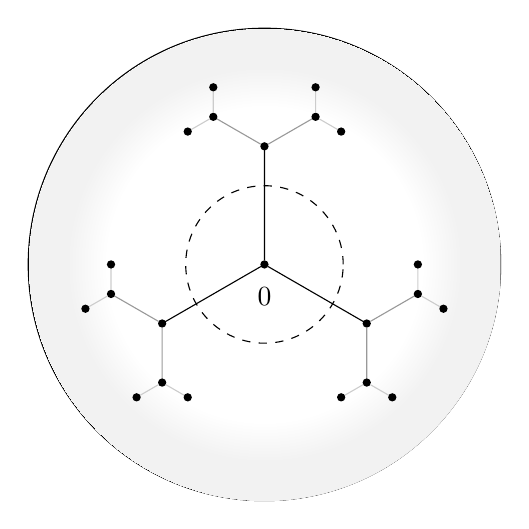
\begin{tikzpicture}[baseline=(current bounding box.center)]
% thanks to Tomasz M. Trzeciak
% based off of http://www.latex-community.org/viewtopic.php?f=4&t=2111

\draw (0,0) circle (3);

\begin{scope}
\pgfsetfading{fading3}{\pgftransformshift{\pgfpoint{0cm}{0cm}}}
\filldraw[black!5] (0,0) circle (3);
\end{scope}

\draw[dashed] (0,0) circle (1);
\coordinate[style={inner sep=0pt, outer sep=0pt, minimum size=3pt, fill=black, circle}] (O) at (0,0);
\node[below=5pt] at (O) {$0$};

\draw (O) -- +( 90:1.5) coordinate[style={inner sep=0pt, outer sep=0pt, minimum size=3pt, fill=black, circle}] (Q1)
      (O) -- +(210:1.5) coordinate[style={inner sep=0pt,outer sep=0pt,minimum size=3pt, fill=black,circle}] (Q2)
      (O) -- +(330:1.5) coordinate[style={inner sep=0pt,outer sep=0pt,minimum size=3pt, fill=black,circle}] (Q3);

\draw[black!40] (Q1) -- +(120-90:0.75) coordinate[style={inner sep=0pt, outer sep=0pt, minimum size=3pt, fill=black, circle}] (Q12)
      (Q1) -- +(240-90:0.75) coordinate[style={inner sep=0pt, outer sep=0pt, minimum size=3pt, fill=black, circle}] (Q13)
      (Q2) -- +(120-330:0.75) coordinate[style={inner sep=0pt, outer sep=0pt, minimum size=3pt, fill=black, circle}] (Q21)
      (Q2) -- +(240-330:0.75) coordinate[style={inner sep=0pt, outer sep=0pt, minimum size=3pt, fill=black, circle}] (Q23)
      (Q3) -- +(120-210:0.75) coordinate[style={inner sep=0pt, outer sep=0pt, minimum size=3pt, fill=black, circle}] (Q31)
      (Q3) -- +(240-210:0.75) coordinate[style={inner sep=0pt, outer sep=0pt, minimum size=3pt, fill=black, circle}] (Q32);

\draw[black!20] (Q12) -- +(90:0.375) coordinate[style={inner sep=0pt, outer sep=0pt, minimum size=3pt, fill=black, circle}] (Q121)
      (Q12) -- +(330:0.375) coordinate[style={inner sep=0pt, outer sep=0pt, minimum size=3pt, fill=black, circle}] (Q123)
      (Q13) -- +(90:0.375) coordinate[style={inner sep=0pt, outer sep=0pt, minimum size=3pt, fill=black, circle}] (Q131)
      (Q13) -- +(210:0.375) coordinate[style={inner sep=0pt, outer sep=0pt, minimum size=3pt, fill=black, circle}] (Q132)
      (Q21) -- +(90:0.375) coordinate[style={inner sep=0pt, outer sep=0pt, minimum size=3pt, fill=black, circle}] (Q212)
      (Q21) -- +(210:0.375) coordinate[style={inner sep=0pt, outer sep=0pt, minimum size=3pt, fill=black, circle}] (Q213)
      (Q23) -- +(210:0.375) coordinate[style={inner sep=0pt, outer sep=0pt, minimum size=3pt, fill=black, circle}] (Q231)
      (Q23) -- +(330:0.375) coordinate[style={inner sep=0pt, outer sep=0pt, minimum size=3pt, fill=black, circle}] (Q232)
      (Q31) -- +(210:0.375) coordinate[style={inner sep=0pt, outer sep=0pt, minimum size=3pt, fill=black, circle}] (Q312)
      (Q31) -- +(330:0.375) coordinate[style={inner sep=0pt, outer sep=0pt, minimum size=3pt, fill=black, circle}] (Q313)
      (Q32) -- +(90:0.375) coordinate[style={inner sep=0pt, outer sep=0pt, minimum size=3pt, fill=black, circle}] (Q321)
      (Q32) -- +(330:0.375) coordinate[style={inner sep=0pt, outer sep=0pt, minimum size=3pt, fill=black, circle}] (Q323);
\end{tikzpicture}%
%
\quad $\xrightarrow{\pi_{GH}}$ \quad%
%
\begin{tikzpicture}[baseline=(current bounding box.center)]

\newcommand\pgfmathsinandcos[3]{%
  \pgfmathsetmacro#1{sin(#3)}%
  \pgfmathsetmacro#2{cos(#3)}%
}
\newcommand\LongitudePlane[3][current plane]{%
  \pgfmathsinandcos\sinEl\cosEl{#2} % elevation
  \pgfmathsinandcos\sint\cost{#3} % azimuth
  \tikzset{#1/.style={cm={\cost,\sint*\sinEl,0,\cosEl,(0,0)}}}
}
\newcommand\DrawLongitudeCircle[2][1]{
  \LongitudePlane{35}{#2} % first argument is angle of elevation
  \tikzset{current plane/.prefix style={scale=#1}}
   % angle of "visibility"
  \pgfmathsetmacro\angVis{atan(sin(#2)*cos(35)/sin(35))} % these are angle of elevation too
  % this might assume that the angle of elevation is positive
  \draw[current plane] (\angVis:1) arc (\angVis:90:1);
  \draw[current plane,dashed] (\angVis:1) arc (\angVis:-90:1);
}

% the "2.5" magic number is the radius of the sphere 
% the "35" magic number is the angle of elevation of the camera
\pgfmathsetmacro\H{2.5*cos(35)}
\filldraw[ball color=white] (0,0) circle (2.5);
\foreach \t in {-5,-125,-245} { \DrawLongitudeCircle[2.5]{\t} }
\coordinate[style={inner sep=0pt,outer sep=0pt,minimum size=3pt,
    fill=black,circle}] (O) at (0,-\H);
\node[below=16pt] at (O) {$0$};
\coordinate[style={inner sep=0pt,outer sep=0pt,minimum size=3pt,
    fill=black,circle}] (I) at (0,\H);
\node[above=16pt] at (I) {$\infty$};
\end{tikzpicture}
\end{center}

\caption{The period map at $n = 2$, $p = 2$}
\end{figure}

\begin{theorem}\citeme{\cite{HopkinsGrossAnnouncement,StricklandGHDuality}}
\todo{Make sure you get this right.}
The sheaf $\context{E_\Gamma}(\mathbb I_{\Q/\Z})$ is the dualizing sheaf on $(\moduli{fg})^\wedge_\Gamma$. \qed
\end{theorem}





\section{Knowns and unknowns}



\subsection*{Higher orientations}

$\TAF$ and friends\label{TAFDiscussion}

The $\alpha_{1/1}$ argument: Prop 2.3.2 of Hovey's $v_n$--elements of ring spectra

% The HLP calculations

\subsection*{Equivariance}

This is tied up with the theory of power operations in a way I've never really thought about.  Seems complicated.

You should also mention the ``rigidity'' of the elliptic genus, which is about an $S^1$--equivariant version.

\subsection*{Index theorems}

Connections with analysis

The Stolz--Teichner program








-----

Contexts for structured ring spectra

Difficulty in computing $\S_d \actson E_d^*$. (Gross--Hopkins and the period map.)

Barry's $p$--adic measures

Fixed point spectra and e.g. $L_{K(2)} \tmf$.

Blueshift, A--M--S, and the relationship to A--F--G?

Does $E_n$ receive an $E_\infty$ orientation?  Does $BP$?

Remark 12.13 of published $H_\infty$ AHS says their obstruction framework agrees with the $E_\infty$ obstruction framework (if you take everything in sight to have $E_\infty$ structures).  This is almost certainly related to the discussion at the end of Matt's thesis about the $MU$--orientation of $E_d$.\todo{Section 12.4 compares doing $H_\infty$ descent with doing $E_\infty$ descent and shows that they're the same (in the case of interest?).}

Hovey's paper on $v_n$--periodic elements in ring spectra.  He has a nice (and thorough!) exposition on why one should be interested in bordism spectra and their splittings: for instance, a careful analysis of $M\Spin$ will inexorably lead one toward studying $KO$.  It would be nice if studying $M\String$ (and potentially higher analogues) would lead one toward non-completed, non-connective versions of $EO_n$.  Talk about $BoP$, for instance.

Matt's short resolutions of chromatically localized $MU$.






\begin{remark}
It is completely unclear why $MU$ plays such an important mediating role between geometry (i.e., the stable category) and algebra (i.e., sheaves on the moduli of formal groups).  Given a general ring spectrum $R$ and thick prime $\otimes$--ideals $\CatOf C_\alpha$ of perfect $R$--modules, one ask the analogous two questions:
\begin{enumerate}
\item Is it possible to find an $R$--algebra $S$ whose context functor induces a homeomorphism of Balmer spectra $\Spec(\CatOf{Modules}_R^{\perf}) \to \Spec(\CatOf{QCoh}(\context{S/R}))$?
\item Are there complementary localizers $L_\alpha\co \CatOf{Modules}_R \to \CatOf{Modules}_{R,(\alpha)}$?  Can they be presented via Bousfield's framework as homological localizations for auxiliary $S$--algebra spectra $S_\alpha$?  Do the contexts $\context{S_\alpha}$ admit compatible localizers with $\context{S}$?
\end{enumerate}
For $R = \S$, this is the role that the $R$--algebra $S = MU$ and the $S$--algebras $S_d = E(d)$ play.  Finding these spectra feels like striking gold, and it is unclear how to produce analogous spectra in general.
\todo{Mathews's work on Galois descent shows that the fixed point map $\CatOf{Modules}_{E_\Gamma, \Aut \Gamma}^{\mathrm{complete}} \to \CatOf{Spectra}_{\Gamma}$ is an equivalence of categories.}
\end{remark}




\begin{remark}
The homotopy of $\widehat L_2 \S$ is also known, by work of Shimomura and collaborators~\cite{Shimomura,ShimomuraYabeM20,ShimomuraYabeL2S} (but see also the reorganization by Behrens~\cite{BehrensRevisited}).  It is \emph{exceedingly} complicated, and it is an open problem to find an expression of it which admits human digestion.  Behrens has pursued a program encoding this problem in terms of modular forms~\cite{BehrensCongruences,BehrensModularDescription,BehrensBuildings}, and Hopkins has proposed a program involving $L$--functions~\cite{StricklandpAdicInterpolation}, motivated by which Hovey and Strickland have shown a kind of continuity result for among the groups~\cite[Section 14]{HoveyStrickland}.
\end{remark}





\begin{remark}
There are also ``finitary'' flavors of chromatic localization available, which are typically less robust but more computable.  They assemble into a diagram:
\begin{center}
\begin{tikzcd}
E \arrow{r} \arrow{d} & L_d^{\fin} E \arrow{r} \arrow{d} & L_d E \arrow{d} \\
L_{X(d)} E \arrow{r} & \widehat L_d^{\fin} E \arrow{r} & \widehat L_d E,
\end{tikzcd}
\end{center}
where $X(d)$ is a finite complex of type exactly $d$, $v$ is a $v_d$--self-map of $X(d)$, $T(d) = X(d)[v^{-1}]$ is the localizing telescope, $\widehat L_d^{\fin}$ is Bousfield localization with respect to $T(d)$ (which can be shown to be independent of choice of $X(d)$ and of $v$), and $L_d^{\fin}$ denotes localization with respect to the class of \emph{finite} $E(d)$--acyclics.  Many things about these functors are known: for instance, $L_{X(d)} L_d = \widehat L_d$, there is a chromatic fracture square relating $L_d^{\fin}$ to $\widehat L_{\le d}^{\fin}$, and $L_d^{\fin} E \simeq L_d E$ if and only if $\widehat L_{\le d}^{\fin} E \simeq \widehat L_{\le d} E$.  One major question about these functors remains open, corresponding the last unsettled nilpotence and periodicity conjecture of Ravenel~\cite[Conjecture 10.5]{RavenelLocalizationWRTPeriodic}: is the map $\widehat L_d^{\fin} E \to \widehat L_d E$ an equivalence?  Multiple proofs and disproofs have been offered, but the literature remains unsettled.
\citeme{Find some proofs and disproofs.}
\end{remark}







\begin{remark}
Writing $M_d$ for the fiber in the sequence $M_d \to L_d \to L_{d-1}$, the filtration spectral sequence associated to the tower in \Cref{ChromaticConvergence} is called the \textit{geometric chromatic spectral sequence}, which has the form $\pi_* M_* \S \Rightarrow \pi_* \S_{(p)}$.  The two forms of filtration data $M_d X$ and $\widehat L_d X$ are actually functorially equivalent to one another:
\begin{align*}
\widehat L_d M_d & \simeq \widehat L_d, &
M_d \widehat L_d & \simeq M_d,
\end{align*}
but they have fairly distinct properties.  For instance, $M_d$ is smashing whereas $\widehat L_d$ is not, $M_d$ is not part of an adjoint pair whereas $\widehat L_d$ is, and the analogue of \Cref{FormulaForKnLocalization} for $M_d$ is ``backwards'':\citeme{I forget who this is due to} \[M_d X \simeq \colim_I \left( M^0(v^I) \sm L_d X \right).\]  The spectrum $M_d X$ also relates to the chromatic fracture square for $X$:
\begin{center}
\begin{tikzcd}
M_d X \arrow{d} \arrow[equal]{r} & M_d X \arrow{d} \\
L_d X \arrow{r} \arrow{d} \arrow[dr, phantom, "\lrcorner", very near start] & \widehat L_d X \arrow{d} \\
L_{d-1} X \arrow{r} & L_{d-1} \widehat L_d X.
\end{tikzcd}
\end{center}
From this, we see that there is a fiber sequence $M_d X \to \widehat L_d X \to L_{d-1} \widehat L_d X$.

The case $d = 1$ gives the prototypical example of the difference between these two presentations of the ``exact height $d$ data'', where the sequence becomes: \[\colim_j (M^0(p^j) \sm L_1 X) \to \lim_j (M_0(p^j) \sm L_1 X) \to \left( \lim_j (M_0(p^j) \sm L_1 X) \right)_{\Q}.\]  If, for instance, $\pi_0 L_1 X = \Z_{(p)}$, then the long exact sequence of homotopy groups associated to this fiber sequence gives
\begin{center}
\begin{tikzcd}
\pi_0 \widehat L_1 X \arrow{r} \arrow[equal]{d} & \pi_0 L_0 \widehat L_1 X \arrow{r} \arrow[equal]{d} & \pi_{-1} M_1 X \arrow[equal]{d} \\
\Z^\wedge_p \arrow{r} & \Q_p \arrow{r} & \Z/p^\infty.
\end{tikzcd}
\end{center}
Coupling this to \Cref{piLK1SExample}, we compute
\begin{align*}
\pi_t M_1 \S^0 & = \begin{cases} \Z/p^\infty & \text{when $t = -1$}, \\ \Z_p / (pk) & \text{when $t = k|v_1| - 1$ and $t = \ne 0$}, \\ \Z/p^\infty & \text{when $t = (0 \cdot |v_1| - 1) - 1 = -2$}, \\ 0 & \text{otherwise}. \end{cases}
\end{align*}
This is a model for what happens generally when passing from $\pi_* \widehat L_d X$ to $\pi_* M_d X$: the $v_j$--torsion--free groups get converted to infinitely $v_j$--divisible groups, with some dimension shifts.\footnote{A height $2$ example of this same phenomenon is visible in Behrens's paper~\cite[Section 7]{BehrensRevisited}.}
\end{remark}



Sections 5.3-4 of Hopkins's ICM address \textit{Algebraic Topology and Modular Forms} has a discussion of what $\eta$ and $\nu$ have to do with $\tmf$, as well as the construction of some interesting ``topological $\theta$--series'' in the elliptic cohomology of certain Thom complexes.



